Das Experiment dient dazu, die physikalischen Gesetze des Luftwiderstand zu erarbeiten und zu erlernen. 

\subsection{Aufbau des Experiments}

Für das Experiment wurden folgende Mittel verwendet:

\begin{itemize}
	\item 1 Entfernungsmesser
	\item 6 Testobjekte in Form von Papierkegel
	\item 1 Rechner zur Aufzeichnung und Speicherung der Ergebnisse des Entfernungsmesser
	\begin{itemize}
		\item Betriebssystem: Windows 10 
		\item Aufzeichnungssoftware: Logger Pro (Trial)
	\end{itemize}
\end{itemize}

Diese wurden wie in der Abbildung \ref{fig:expsetup} angeordnet.

\subsection{Ablauf des Experiments}



\begin{figure}
	\center
	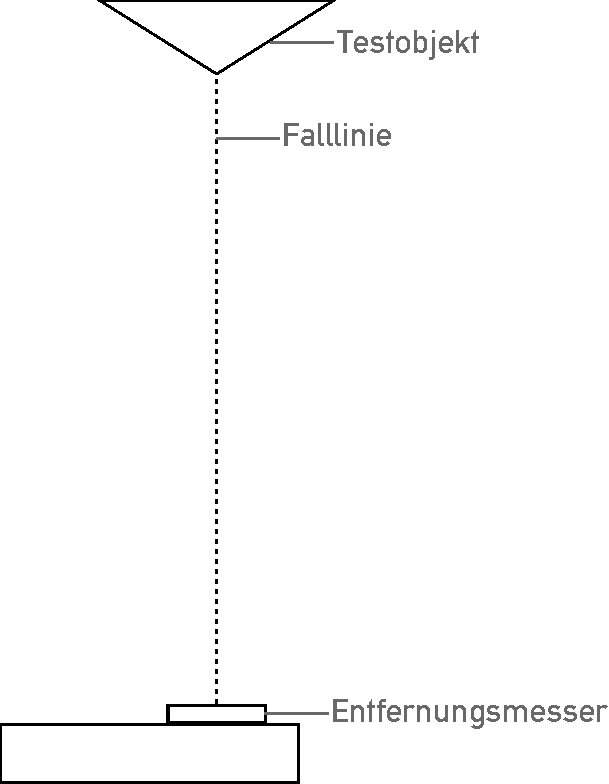
\includegraphics[width=5cm]{diagrams/experiment_aufbau}\caption{\label{fig:expsetup} Aufbau des Experiments}	
\end{figure}
